\documentclass[11pt, a4paper]{book}
% Ressources à installer : texlive-science et texlive-lang-french ou texlive-lang-european
%à compiler avec XeLaTeX à cause des image pstricks

\usepackage[utf8]{inputenc}
\usepackage[T1]{fontenc}

\usepackage[french]{babel}
\usepackage{listingsutf8}
\usepackage{pdfpages}
\usepackage{tikz,pgf}
\usepackage{amsthm,titlesec}
\usepackage{mdframed} % pour le format des définition, théorèmes...
\usepackage{xcolor,rotating,systeme}
\usepackage[Glenn]{fncychap} %pour le format des chapitres
\usepackage[top=3cm,bottom=3cm,left=3cm,right=2cm,headsep=10pt,a4paper]{geometry} % Page margins
\usepackage{multicol}
\usepackage{comment}
\usepackage{enumerate,cancel}
\usepackage{lipsum,minitoc}
%\usepackage{chngcntr}
\usepackage{amsmath,amsfonts,minitoc,amsthm,pgfplots}
\usepackage{mathrsfs}
\usetikzlibrary{arrows, intersections}
\usepackage{mathrsfs}
\usepackage{array,yhmath}
\usepackage{hyperref}
\usepackage{caption}
\usepackage{float}
\usepackage{wrapfig}
\restylefloat{figure}
%\usepackage{subfig}

\usepackage{subcaption}

\usepackage{listings}
\usepackage{color}
\lstset{ % General setup for the package
    language=Python,
    basicstyle=\footnotesize,
    basewidth=0.7em,
    numbers=left,
     numberstyle=\tiny,
    frame=lines,
    tabsize=4,
    columns=fixed,
    showstringspaces=false,
    showtabs=false,
    keepspaces,
    commentstyle=\color{gray},
    keywordstyle=\color{blue},
    stringstyle=\color{magenta},
    inputencoding=utf8/latin1,
            extendedchars=true,
            literate=%
            {é}{{\'{e}}}1
            {è}{{\`{e}}}1
            {ê}{{\^{e}}}1
            {ë}{{\¨{e}}}1
            {û}{{\^{u}}}1
            {ù}{{\`{u}}}1
            {â}{{\^{a}}}1
            {à}{{\`{a}}}1
            {î}{{\^{i}}}1
            {ô}{{\^{o}}}1
            {ç}{{\c{c}}}1
            {Ç}{{\c{C}}}1
            {É}{{\'{E}}}1
            {Ê}{{\^{E}}}1
            {À}{{\`{A}}}1
            {Â}{{\^{A}}}1
            {Î}{{\^{I}}}1
    }



\usepackage{lipsum}
\newtheorem{example}{Exemple}

\usepackage{pstricks,pst-plot,pstricks-add}
\usepackage{pst-func,tkz-tab,tkz-euclide}
\usepackage{graphicx}
%macro exo
\newcounter{mtex}[chapter]
\newcommand{\mtexlabel}{\cadrexo{\themtex}}
\newcommand{\cadrexo}[1]{%
\tikz\node[rectangle,minimum size=6mm,rounded corners=2mm,fill=ocre,inner sep=0pt,text width=0.8cm,align=center]{\large\bfseries\textcolor{white}{#1}};}
\definecolor{ocre}{RGB}{196,106,106}
\definecolor{vert}{RGB}{55,120,0}
\newcommand{\mtexlabelpos}[1]{%
\makebox[0pt][r]{\raisebox{#1\baselineskip}[0pt][0pt]{\mtexlabel\quad}}}
\newenvironment{exercice}[1][\empty]{%
\refstepcounter{mtex}%
\trivlist\item\relax%  
\ifx#1\empty\mtexlabelpos{-.7}\else\mtexlabelpos{-.5}%
\hfill\textbf{#1}\hfill\mbox{}\par\fi%
}{\endtrivlist}

\newcommand{\N}{\mathbb{N}}
\newcommand{\Z}{\mathbb Z}
\newcommand{\Q}{\mathbb Q}
\newcommand{\R}{\mathbb R}
\newcommand{\C}{\mathbb C}

\newcommand{\ssi}{\;\;\Leftrightarrow\;\;}

\newcommand{\point}[1]{-- +(#1,#1) -- +(-#1,-#1) -- +(0,0) -- +(-#1,#1) -- +(#1,-#1)} 


\newcommand{\parallele}{\mathbin{\!/\mkern-5mu/\!}} %signe parallèle

\titleformat{\chapter}[frame]
{\setlength\fboxrule{2.25pt}\color{black}}%
{\filleft\scshape\LARGE%
\enspace  Chapitre \thechapter\enspace}%
{20pt}
{\rule{0pt}{30pt}\Huge\scshape\filleft}

\newcommand\fonction[5]{
$\begin{array}{rrll}
#1: & #2 & \rightarrow & #3 \\
  & #4 & \mapsto & #5
\end{array}$
}

%\titleformat
%{\section} % command
%[hang] % shape
%{\bfseries\Large} % format
%{ \thesection\quad} % label
%{0em} % sep
%{
%} % before-code
%[
%\vspace{-1ex}%
%\textcolor{blue!60}{\rule{10cm}{3pt}}
%] % after-code


%\theoremstyle{break}
\newtheoremstyle{definition-style}  %style des theoreme
{}               
{}               
{}                   
{}                   
{\bf\sffamily} 
{~:\\[0.3cm]}                 
{.5em}               
{\thmname{#1}\thmnumber{ #2}\thmnote{ (#3)}}

\mdfdefinestyle{defi-frame}{
linewidth=10pt, %
linecolor= blue!50, % 
backgroundcolor= blue!20,
topline=false, %
bottomline=false, %
rightline=false,%
leftmargin=0pt, %
innerleftmargin=15pt, %
innerrightmargin=1em, 
rightmargin=0pt, % 
innertopmargin=-2pt,%
innerbottommargin=6pt, % 
splittopskip=\topskip, %
%splitbottomskip=\topskip, %
}% 

\mdfdefinestyle{methode-frame}{
	linewidth=10pt, %
linecolor= gray!70, % 
backgroundcolor= white,
topline=false, %
bottomline=false,%
rightline=false,%
leftmargin=0pt, %
innerleftmargin=15pt, %
innerrightmargin=1em, 
rightmargin=0pt, % 
innertopmargin=-2pt,%
innerbottommargin=6pt, % 
splittopskip=\topskip, %
%splitbottomskip=\topskip, %
}% 


\mdfdefinestyle{thm-frame}{
linewidth=10pt, %
linecolor= red!50, % 
backgroundcolor= orange!30,
topline=false, %
bottomline=false, %
rightline=false,%
leftmargin=0pt, %
innerleftmargin=15pt, %
innerrightmargin=1em, 
rightmargin=0pt, % 
innertopmargin=-2pt,%
innerbottommargin=6pt, % 
splittopskip=\topskip, %
%splitbottomskip=\topskip, %
}% 

\mdfdefinestyle{lem-frame}{
linewidth=10pt, %
linecolor= yellow!50, % 
backgroundcolor= yellow!10,
topline=false, %
bottomline=false, %
rightline=false,%
leftmargin=0pt, %
innerleftmargin=15pt, %
innerrightmargin=1em, 
rightmargin=0pt, % 
innertopmargin=-2pt,%
innerbottommargin=6pt, % 
splittopskip=\topskip, %
%splitbottomskip=\topskip, %
}% 

\mdfdefinestyle{notation-frame}{
linewidth=10pt, %
linecolor= blue!30, % 
backgroundcolor= blue!10,
topline=false, %
bottomline=false, %
rightline=false,%
leftmargin=0pt, %
innerleftmargin=15pt, %
innerrightmargin=1em, 
rightmargin=0pt, % 
innertopmargin=-2pt,%
innerbottommargin=6pt, % 
splittopskip=\topskip, %
%splitbottomskip=\topskip, %
}% 

\mdfdefinestyle{remarque-frame}{
linewidth=0pt, %
linecolor= black!0, % 
backgroundcolor= blue!0,
topline=false, %
bottomline=false, %
rightline=false,%
leftmargin=0pt, %
innerleftmargin=25pt, %
innerrightmargin=25pt, 
rightmargin=0pt, % 
innertopmargin=-2pt,%
innerbottommargin=6pt, % 
splittopskip=\topskip, %
%splitbottomskip=\topskip, %
}% 
\surroundwithmdframed[style=defi-frame]{defi}

\surroundwithmdframed[style=thm-frame]{thm}

\surroundwithmdframed[style=lem-frame]{lem}

\surroundwithmdframed[style=notation-frame]{notation}

\surroundwithmdframed[style=remarque-frame]{remarque}

\surroundwithmdframed[style=remarque-frame]{remarques}

\surroundwithmdframed[style=methode-frame]{methode}

\theoremstyle{definition-style}

%pour avoir un compteur commun a remarque et remarques
\newcounter{compteurremarque}[chapter]
\renewcommand{\thecompteurremarque}{\arabic{compteurremarque}} %définition de l'affichage du compteur

\newtheorem{defi}{Définition}[chapter]
\renewcommand{\thedefi}{\arabic{defi}} %pour ne pas avoir le numéro du chapitre dans la numération de la def
\newtheorem{thm}{Théorème}[chapter]
\renewcommand{\thethm}{\arabic{thm}}
\newtheorem{lem}{Lemme}[chapter]
\renewcommand{\thelem}{\arabic{lem}}
\newtheorem{notation}{Notation}[chapter]
\renewcommand{\thenotation}{\arabic{notation}}
%\newtheorem{remarque}{Remarque}[chapter]
%\renewcommand{\theremarque}{\arabic{remarque}}
%\newtheorem{remarques}{Remarques}[chapter]
%\renewcommand{\theremarques}{\arabic{remarques}}
\newtheorem{methode}{Méthode}[chapter]
\renewcommand{\themethode}{\arabic{methode}}


\newtheorem{remarque}[compteurremarque]{Remarque}
\newtheorem{remarques}[compteurremarque]{Remarques} %remarque et remarques prennent compteurremarque comme compteur commun

\lstMakeShortInline[columns=fixed]|

%%%%%%%% Commandes de Matthieu

%-------------------------------------------------------------------------------
%---- Eclairage : en encadré sur fond jaune avec symbôle "ampoule" à gauche ----
%-------------------------------------------------------------------------------
\definecolor{coleclairage}{RGB}{255 , 221 , 156}
\definecolor{contoureclairage}{RGB}{255 , 192 , 0}
\newenvironment{eclairage}
{
	\begin{center}%
		\begin{tikzpicture}%
			\node[rectangle, draw=contoureclairage, top color=coleclairage!50, bottom color=coleclairage!140, rounded corners=5pt, inner xsep=5pt, inner ysep=6pt, outer ysep=10pt]\bgroup                     
			\begin{minipage}{0.98\linewidth}
				\begin{minipage}{0.08\linewidth}\centerline{
\includegraphics[scale=1]{images/Symbole_eclairage.png}}\end{minipage}
				\begin{minipage}{0.89\linewidth}\itshape\footnotesize
				}
				{                		
				\end{minipage}
			\end{minipage}\egroup;%
		\end{tikzpicture}%
	\end{center}%
}



\newcommand{\putfigure}[6]{
    \begin{minipage}{#1\textwidth}
    \centering
        \includegraphics[width=#2\textwidth,height=#3\textheight]{#4}
        \captionof{figure}{#5}
        \label{#6}
    \end{minipage}
}


\newcommand{\itemb}[1]{\item \textbf{#1}}



%-------------------------------------------------------------------------------
%---- apprendre : en encadré sur fond jaune avec symbole "ampoule" à gauche ----
%-------------------------------------------------------------------------------
\definecolor{colapprendre}{RGB}{50,205,50}
\definecolor{contourapprendre}{RGB}{34,139,34}
\newenvironment{apprendre}
{
	\begin{center}%
		\begin{tikzpicture}%
			\node[rectangle, draw=contourapprendre, top color=colapprendre!10, bottom color=colapprendre!50, rounded corners=5pt, inner xsep=5pt, inner ysep=6pt, outer ysep=10pt]\bgroup                     
			\begin{minipage}{0.98\linewidth}
				\begin{minipage}{0.08\linewidth}\centerline{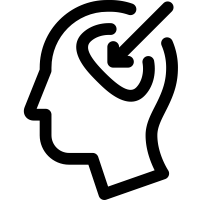
\includegraphics[width=30px]{images/Symbole_learn.png}}\end{minipage}
				\begin{minipage}{0.89\linewidth}\itshape\footnotesize
				}
				{                		
				\end{minipage}
			\end{minipage}\egroup;%
		\end{tikzpicture}%
	\end{center}%
}

\definecolor{colimportant}{RGB}{247 , 189 , 164}
\definecolor{contourimportant}{RGB}{237 , 125 , 49}
\newenvironment{important}
{
	\begin{center}%
		\begin{tikzpicture}%
			\node[rectangle, draw=contourimportant, top color=colimportant!50, bottom color=colimportant!140, rounded corners=5pt, inner xsep=5pt, inner ysep=6pt, outer ysep=10pt]\bgroup                     
			\begin{minipage}{0.08\linewidth}\centerline{
\includegraphics[scale=0.8]{images/Symbole_attention.png}}\end{minipage}
			\begin{minipage}{0.89\linewidth}
			}
			{                		
			\end{minipage}\egroup;
		\end{tikzpicture}%
	\end{center}%
}

%----------------------------------------------
\newcounter{compteurmonprogramme}
\setcounter{compteurmonprogramme}{1}
\newenvironment{monprogramme}
{
	\begin{center}%
		\begin{tikzpicture}%
			\node[rectangle, draw=black, rounded corners=5pt, inner xsep=5pt, inner ysep=6pt, outer ysep=10pt]\bgroup                     
			\begin{minipage}{0.98\linewidth}
				{\bf Programme \thechapter.\thecompteurmonprogramme\;:}
				
				\vspace{2mm}\hspace{7.5mm}
				\begin{minipage}{0.93\linewidth}
				}
				{                		
				\end{minipage}
				\stepcounter{compteurmonprogramme}
			\end{minipage}\egroup;%
		\end{tikzpicture}%
	\end{center}%
}



%------------------------------------------------
%---- Définition : en encadré sur fond blanc ----
%------------------------------------------------
\newcounter{compteurdef}
\setcounter{compteurdef}{1}
\newenvironment{mydefinition}
{
	\begin{center}%
	\begin{tikzpicture}%
		\node[rectangle, draw=black, rounded corners=5pt, inner xsep=5pt, inner ysep=6pt, outer ysep=10pt]\bgroup                    
		\begin{minipage}{0.98\linewidth}
			{\bf {\underline {Définition \thechapter.\thecompteurdef}}}
			
			\vspace{2mm}\hspace{4.5mm}
			\begin{minipage}{0.93\linewidth}
			}
			{                		
			\end{minipage}
			\stepcounter{compteurdef}
		\end{minipage}\egroup;%
	\end{tikzpicture}%
\end{center}%
}

\newenvironment{mydefinitions}
{
	\begin{center}%
		\begin{tikzpicture}%
			\node[rectangle, draw=black, rounded corners=5pt, inner xsep=5pt, inner ysep=6pt, outer ysep=10pt]\bgroup                    
			\begin{minipage}{0.98\linewidth}
				{\bf {\underline {Définitions \thechapter.\thecompteurdef}}}
				
				\vspace{3mm}\hspace{4.5mm}
				\begin{minipage}{0.93\linewidth}\slshape
					\begin{itemize}\setlength{\itemsep}{1mm}
					}
					{                		
				\end{itemize}\end{minipage}
				\stepcounter{compteurdef}
			\end{minipage}\egroup;%
		\end{tikzpicture}%
	\end{center}%
}



%------------------------------------------------
%---- Exemple : en encadré sur fond blanc ----
%------------------------------------------------
\newcounter{compteurex}
\setcounter{compteurex}{1}
\newenvironment{myexample}{
	\begin{center}
	\vspace{-3mm}
	\begin{minipage}{1\linewidth}
		\vspace{2mm}
		{\textsl {\underline {Exemple \thechapter.\thecompteurex}}}
		
		\vspace{2mm}\hspace{2.5mm}
		\begin{minipage}{1\linewidth}
			\begin{mdframed}[topline=false,rightline=false,bottomline=false]
}
{
			\end{mdframed}
		\end{minipage}
		\stepcounter{compteurex}
	\end{minipage}
	\end{center}
}
\newenvironment{myexamples}{
	\begin{center}
		\vspace{-3mm}
		\begin{minipage}{1\linewidth}
			\vspace{2mm}
			{\textsl {\underline {Exemples \thechapter.\thecompteurex}}}
			
			\vspace{2mm}\hspace{2.5mm}
			\begin{minipage}{1\linewidth}%\slshape
				\begin{mdframed}[topline=false,rightline=false,bottomline=false]
					\begin{enumerate}\setlength{\itemsep}{1mm}
				}
				{
					\end{enumerate}
				\end{mdframed}
			\end{minipage}
			\stepcounter{compteurex}
		\end{minipage}
	\end{center}
}



\newtheorem*{question}{Question}



%%%%%%%%%%%%%%%%%%%%%%%%%%%%%%%%%%%%%%%%%%%%%%%%%%%%%%%%%%%%%%%%%%%%%%%%%%%%
%%%%%%%%%%%%%%%%%%%%%%%%%%%   LABELS activite   %%%%%%%%%%%%%%%%%%%%%%%%%%%
%%%%%%%%%%%%%%%%%%%%%%%%%%%%%%%%%%%%%%%%%%%%%%%%%%%%%%%%%%%%%%%%%%%%%%%%%%%%
\newcommand{\act}{\textbf{\textsl{Activité \arabic{compteuract}}} \vspace*{1mm}\\ \addtocounter{compteuract}{1}}
\newcommand{\actnomme}[1]{{\bf Activité \arabic{compteuract} {\textsl{\small (#1)}}}\vspace*{1mm}\\  \addtocounter{compteuract}{1}}
\newcounter{compteuract}
\setcounter{compteuract}{1}
\newcommand{\getactcompteur}{{\the\numexpr \arabic{compteuract} - 1 \relax}}



%%%%%%%%%%%%%%%%%%%%%%%%%%%%%%%%%%%%%%%%%%%%%%%%%%%%%%%%%%%%%%%%%%%%%%%%%%%%
%%%%%%%%%%%%%%%%%%%%%%%%%%%   LABELS EXERCICES   %%%%%%%%%%%%%%%%%%%%%%%%%%%
%%%%%%%%%%%%%%%%%%%%%%%%%%%%%%%%%%%%%%%%%%%%%%%%%%%%%%%%%%%%%%%%%%%%%%%%%%%%
\newcommand{\exo}{\textbf{\textsl{Exercice \arabic{compteurexo}}} \vspace*{1mm}\\ \addtocounter{compteurexo}{1}}
\newcommand{\exonomme}[1]{{\bf Exercice \arabic{compteurexo} {\textsl{\small (#1)}}}\vspace*{1mm}\\  \addtocounter{compteurexo}{1}}
\newcommand{\eexo}{\vspace{5mm}} % espace pour séparer les exercices
\newcounter{compteurexo}
\setcounter{compteurexo}{1}
\newcommand{\getexocompteur}{{\the\numexpr \arabic{compteurexo} - 1 \relax}}
\pgfplotsset{compat=1.17}




\begin{document}
\setcounter{chapter}{6}
\chapter{Réseaux informatiques}

\section{Introduction}


\subsection{Activité 1}

Par groupe de 4 à 6 élèves autour d'une même table.

\ 

{\bf Objectif:} Trouver la méthode la plus simple pour que chaque élève puisse envoyer un message à un autre élève autour de la table.  

\ 

Proposition:

\vskip+3cm

Solution:

\vskip+3cm

Difficultés:

\vskip+3cm

\subsection{Activité 2}
Par groupe de 4 à 6 élèves autour d'une même table.

\ 

{\bf Contrainte:} Chaque élève établit la liste des élèves auxquels il peut envoyer un message. Pour chaque nom inscrit, il doit payer 10 francs. Le {\it prix total de la table} consiste à additionner le prix des listes de chaque élève autour de la table.

\ 

\begin{remarque}
Pour illustrer la contrainte, imaginons que 4 personnes, nommées {\it A}, {\it B}, {\it C} et {\it D} se trouvent autour de la table. {\it A} met sur sa liste {\it C} et {\it D} ({\it A} peut donc envoyer un message à {\it C} et {\it D } mais pas  {\it C}). {\it B} met sur sa liste {\it A}. {\it C} met sur sa liste {\it A} et {\it B}. {\it D} ne met personne sur sa liste. 

Le prix total de la table est donc: $2 \cdot 10 + 1 \cdot 10 + 2 \cdot 10 + 0 \cdot 10=50 Frs$ 

\end{remarque}
\ 

{\bf Objectif:} Trouver une méthode simple pour que chaque élève puisse envoyer un message à un autre élève autour de la table {\bf et} que le {\it prix total de la table} soit le plus bas possible.

\ 

Proposition :

\vskip+3cm

Solution:

\vskip+3cm

Difficultés:

\vskip+3cm


\subsection{Activité 3}
Par groupe de 4 à 6 élèves autour d'une même table.

\ 

{\bf Contrainte:} Si un élève $A$ peut envoyer un message à un élève $B$ alors $B$ peut aussi en envoyer à $A$ : si $A$ a inscrit $B$ sur sa liste alors $B$ a aussi inscrit $A$ sur sa liste.

\ 

{\bf Objectif:} Trouver une méthode simple pour que chaque élève puisse envoyer un message à un autre élève autour de la table {\bf et} que le {\it prix total de la table} soit le plus bas possible.

\ 

Proposition :

\vskip+3cm

Solution:

\vskip+3cm

Difficultés:

\vskip+3cm





\subsection{Activité 4}

Par groupe de 4 à 6.

\ 

{\bf Objectif:} Trouver une méthode simple pour que chaque élève puisse envoyer un message à un autre élève {\bf dans la classe} et que le prix total de la classe soit le plus bas possible.

\ 

Proposition :

\vskip+3cm

Solution:

\vskip+3cm

Difficultés:

\vskip+3cm

\newpage

\section{Réseaux et graphes}
\subsection{Définition}

\begin{defi}
Un {\bf réseau informatique} est un ensemble d'équipements reliés entre eux pour échanger des informations.
\end{defi}

\ 
\begin{exercice}
Quels exemples de réseaux connaissez-vous?

\end{exercice}

\subsection{Les types de réseaux}

\subsubsection{Les réseaux personnels}

Les {\bf réseaux personnels} ou {\bf PAN (Personnal Area Network)} en anglais, permettent à des appareils de communiquer entre eux à l'échelle d'une personne. Il couvre des distances ne dépassant pas quelques mètres. Un exemple de PAN est la technologie {\it bluetooth} permettant de connecter une souris ou un clavier à un ordinateur.

\subsubsection{Les réseaux locaux}

Les {\bf réseaux locaux} ou {\bf LAN (Local Area Network)} en anglais, correspondent aux réseaux privés: chez les particuliers, dans les entreprises, les écoles, les universités, les administrations... Ils couvrent le plus souvent des distances allant d'une dizaine à une centaine de mètres. Un exemple est le réseau Wi-Fi d'une habitation. 

\subsubsection{Les réseaux étendus}

Les {\bf réseaux étendus} ou {\bf WAN (Wide Area Network)} en anglais,  sont les réseaux qui couvrent de vastes régions géographiques, telles qu'un pays ou un continent. Ils couvrent des distances allant jusqu'à plusieurs milliers de kilomètres. Un exemple de WAN est le réseau privé d'une entreprise qui connecte ses différentes branches dans un pays.

\subsubsection{Les inter-réseaux}

Les {\bf inter-réseaux} ou {\bf internetwork} en anglais sont les réseaux les plus connus puisque Internet fait partie de cette catégorie. Comme l'indique leur nom, ces réseaux connectent plusieurs sous-réseaux  qui peuvent être de taille et de nature différentes. Ils couvrent de grandes zones géographiques, comme c'est le cas d'Internet.

\begin{exercice}
Dans quel type de réseaux se classent les réseaux suivants?
\begin{enumerate}
\item Le réseau Wi-Fi dans le fast-food où je mange.
\item Ma manette de jeu sans fil connecté à ma console de jeu.
\item Le réseau connectant toutes les succursales Toyota.
\item Le réseau connectant les postes suisses.
\item Le réseau de l'université de Genève.
\item Internet.
\item Mon téléphone connecté à mon ordinateur pour transférer des photos. 

\end{enumerate}



\end{exercice}




\subsection{Graphes}

Afin de bien représenter les différents types de réseaux, nous avons besoin de définir une structure spécifique, qui se nomme le {\bf graphe}:

\begin{defi}
Un {\bf graphe} est une structure de données composée de {\bf noeuds}, qui représentent les entités avec lesquelles on travaille, et d'{\bf arcs} qui représentent les connections entre les noeuds.

\end{defi}

Par exemple, si nous avons 4 élèves nommés {\it A}, {\it B}, {\it C} et  {\it D} et que nous voulons que  {\it A} soit relié à  {\it B} et  {\it D}, et que  {\it D} soit relié à  {\it B} et  {\it C} alors nous pouvons représenter cette situation par le graphe suivant:



\begin{center}
\begin{tikzpicture}[scale=.45]
\filldraw[fill=lightgray] (0,0) circle (1cm);
\draw (0,0) node {$A$};

\filldraw[fill=lightgray] (6,0) circle (1cm);
\draw (6,0) node {$B$};

\filldraw[fill=lightgray] (6,6) circle (1cm);
\draw (6,6) node {$C$};

\filldraw[fill=lightgray] (0,6) circle (1cm);
\draw (0,6) node {$D$};

\draw[thick] (1,0) -- (5,0);
\draw[thick] (0,1) -- (0,5);
\draw[thick] (1,6) -- (5,6);
\draw[thick] (1.41/2,6-1.41/2) -- (6-1.41/2,1.41/2);



\end{tikzpicture}
\end{center}


Ce graphe a 4 nœuds et 4 arcs. Un arc peut être noté $(A;B)$ pour signifié qu'il y a une connexion entre les nœuds $A$ et $B$.

\begin{exercice}
Tracer les graphes suivants:
\begin{enumerate}
\item Un graphe avec 5 nœuds  nommés $A$, $B$, $C$, $D$ et $E$ et tel que $A$ et $E$ soient connectés à tous les autres nœuds.
\item Un graphe avec 6 nœuds  nommés $A$, $B$, $C$, $D$, $E$ et $F$ et avec les arcs suivants: $(A;B)$, $(B;C)$, $(C;D)$, $(D;E)$ et $(E;A)$.
\item Un graphe avec 4 nœuds  $A$, $B$, $C$ et $D$ et chaque nœud est connecté à tous les autres nœuds.

\end{enumerate}

\end{exercice}


\section{Topologies des réseaux}

\subsection{Définition}

\begin{defi}
La {\bf topologie} d'un réseau décrit la façon dont sont connectés ses nœuds entre eux.
\end{defi}



\subsection{Topologie en bus}

\begin{defi}
Dans un {\bf réseau en bus} tous les nœuds du réseau sont connectés au même support (un câble par exemple), appelé bus. Lorsqu’un nœud envoie de l'information sur le bus, tous les autres nœuds la reçoivent.
\end{defi}

Par exemple, le graphe suivant représente 5 appareils connecté en réseau en bus. 

\begin{center}
\begin{tikzpicture}[scale=.5]
\filldraw[fill=lightgray] (0,0) circle (1cm);
%\draw (0,0) node {$A$};

\filldraw[fill=lightgray] (4,0) circle (1cm);
%\draw (6,0) node {$B$};

\filldraw[fill=lightgray] (8,0) circle (1cm);
%\draw (6,6) node {$C$};

\filldraw[fill=lightgray] (12,0) circle (1cm);

\filldraw[fill=lightgray] (16,0) circle (1cm);
%\draw (0,6) node {$D$};

\draw[thick] (0,1) -- (0,4);
\draw[thick] (4,1) -- (4,4);
\draw[thick] (8,1) -- (8,4);
\draw[thick] (12,1) -- (12,4);
\draw[thick] (16,1) -- (16,4);

\filldraw[fill=lightgray] (-1,3) rectangle (17,4);

\draw (8,3.5) node {Bus};




\end{tikzpicture}
\end{center}


\begin{remarques}
\begin{enumerate}
\item[]
\item {\bf Avantages} : 
	\begin{enumerate}
		\item Tous les appareils sont connectés entre eux et peuvent donc communiquer directement.
		\item  Facile à mettre en œuvre et fonctionnement simple.
		\item Ajout d'un appareil facile.\\
	\end{enumerate}
\item {\bf Désavantages} :
	\begin{enumerate}
		\item Une rupture de câble produit une déconnexion des appareils.
		\item Les collisions (plusieurs informations simultanées mises sur le bus) sont fréquentes.
		\item Plus il y a d'appareils connectés, plus il y a une baisse des performances du réseau.
	\end{enumerate}
\end{enumerate}
\end{remarques}












\subsection{Topologie en étoile}


\begin{defi}
Dans un {\bf réseau  en étoile} les nœuds du réseau sont tous connectés à un même appareil central appelé {\bf concentrateur} ({\bf hub} en anglais) ou {\bf commutateur} ({\bf switch} en anglais). Le rôle de cet appareil central est de gérer les communications entre les appareils connectés au réseau.
\end{defi}

Par exemple, le graphe suivant représente un réseau en étoile avec 6 appareils connectés à un concentrateur.


\begin{center}
\begin{tikzpicture}[scale=.5]

\draw (-4,0) -- (4,0);
\draw (-2,3.8) -- (2,-3.8);
\draw (-2,-3.8) -- (2,3.8);

\filldraw[fill=lightgray] (0,0) circle (1.2cm);
%\draw (0,0) node {$A$};



\filldraw[fill=lightgray] (4,0) circle (1cm);
%\draw (6,0) node {$B$};

\draw (0,0) node {hub};

\filldraw[fill=lightgray] (-4,0) circle (1cm);
%\draw (6,6) node {$C$};

\filldraw[fill=lightgray] (-2,3.8) circle (1cm);

\filldraw[fill=lightgray] (2,3.8) circle (1cm);

\filldraw[fill=lightgray] (-2,-3.8) circle (1cm);

\filldraw[fill=lightgray] (2,-3.8) circle (1cm);





\end{tikzpicture}
\end{center}



\begin{remarques}
\begin{enumerate}
\item[]
\item {\bf Avantages} : 
	\begin{enumerate}
		\item Tous les appareils communiquent entre eux aisément, le risque de collision est réduit.
		\item  La panne d'un appareil ne réduit pas l'efficacité du réseau.
		\item L'ajout d'un appareil est facile.\\
	\end{enumerate}
\item {\bf Désavantages} :
	\begin{enumerate}
		\item Il est plus coûteux qu'en réseau en bus car nécessite un concentrateur ou un commutateur.
		\item L'efficacité du réseau est conditionné au bon fonctionnement du concentrateur ou du commutateur.
	\end{enumerate}
\end{enumerate}
\end{remarques}



\subsection{Topologie en anneau}
\begin{defi}
Dans un {\bf réseau en anneau}, chaque appareil est connecté à deux appareils avec lesquels il peut communiquer, formant ainsi une boucle.

\noindent Un ordinateur n'accepte une information que si elle lui est destinée sinon il fait passer l'information à l'ordinateur suivant.
\end{defi}

Par exemple, le graphe suivant représente un réseau de 6 appareils connectés en anneau.




\begin{center}
\begin{tikzpicture}[scale=.5]

\draw (-4,0) -- (-2,3.8) -- (2,3.8) -- (4,0) -- (2,-3.8) -- (-2,-3.8) -- cycle;



%\draw (0,0) node {$A$};



\filldraw[fill=lightgray] (4,0) circle (1cm);
%\draw (6,0) node {$B$};



\filldraw[fill=lightgray] (-4,0) circle (1cm);
%\draw (6,6) node {$C$};

\filldraw[fill=lightgray] (-2,3.8) circle (1cm);

\filldraw[fill=lightgray] (2,3.8) circle (1cm);

\filldraw[fill=lightgray] (-2,-3.8) circle (1cm);

\filldraw[fill=lightgray] (2,-3.8) circle (1cm);





\end{tikzpicture}
\end{center}



\begin{remarques}
\begin{enumerate}
\item[]
\item {\bf Avantages} : 
	\begin{enumerate}
		\item Le nombre de câbles est réduit.
		\item Il y a absence de collision.
		\item Le réseau est fiable.\\
	\end{enumerate}
\item {\bf Désavantages} :
	\begin{enumerate}
		\item La panne de deux ordinateurs arrête le réseau.
		\item L'ajout ou la suppression d'un ordinateur paralyse le système.
	\end{enumerate}
\end{enumerate}
\end{remarques}


\subsection{Topologie maillée}

\begin{defi}
Dans un {\bf réseau maillé} les appareils sont connectés les uns aux autres de manière arbitraire.

\noindent Lorsqu’un nœud veut envoyer un message à un autre, il doit trouver un chemin à travers le réseau pour que l’information puisse atteindre sa destination.
\end{defi}

Par exemple, le graphe suivant représente un réseau maillé avec 8 noeuds et 11 arcs.

\begin{center}
\begin{tikzpicture}[scale=.5]

\coordinate (A) at (-4,0);
\coordinate (B) at (-2,3);
\coordinate (C) at (-2,-3);
\coordinate (D) at (0,0);
\coordinate (E) at (2,3);
\coordinate (F) at (2,-3);
\coordinate (G) at (4,0);
\coordinate (H) at (6,3);

\draw (A) -- (B);
\draw (A) -- (C);
\draw (A) -- (D);
\draw (D) -- (G);
\draw (D) -- (H);
\draw (E) -- (H);
\draw (G) -- (H);
\draw (G) -- (F);
\draw (F) -- (A);
\draw (F) -- (C);
\draw (F) -- (D);



\filldraw[fill=lightgray] (C) circle (1cm);
%\draw (6,0) node {$B$};


\filldraw[fill=lightgray] (0,0) circle (1cm);
%\draw (6,0) node {$B$};

\filldraw[fill=lightgray] (-4,0) circle (1cm);
%\draw (6,6) node {$C$};

\filldraw[fill=lightgray] (4,0) circle (1cm);

\filldraw[fill=lightgray] (2,3) circle (1cm);

\filldraw[fill=lightgray] (6,3) circle (1cm);

\filldraw[fill=lightgray] (2,-3) circle (1cm);

\filldraw[fill=lightgray] (-2,3) circle (1cm);

\filldraw[fill=lightgray] (-2,3) circle (1cm);





\end{tikzpicture}
\end{center}



\begin{remarques}
\begin{enumerate}
\item[]
\item {\bf Avantages} : 
	\begin{enumerate}
		\item La panne d'un câble ou d'un appareil n'influence pas l'efficacité du réseau.
		\item Il est possible de connecter beaucoup d'appareils.\\
	\end{enumerate}
\item {\bf Désavantages} :
	\begin{enumerate}
		\item Un réseau maillé nécessite une stratégie pour envoyer les informations au bon destinataire.
		\item Un réseau maillé nécessite de nombreuses connexions pour augmenter sa fiabilité.
	\end{enumerate}
\end{enumerate}
\end{remarques}







\subsection{Topologie maillé complètement}

C'est le réseau le plus évident. Lorsque deux appareils veulent communiquer, ils s'envoient directement les informations car ils sont connectés l'un à l'autre. 

\begin{defi}
Dans un {\bf réseau  maillé complètement} tous les nœuds sont connectés à tous les autres. Dans ce cas, les nœuds peuvent communiquer directement entre eux, sans passer par aucun intermédiaire.
\end{defi}

\ 

Par exemple, le graphe suivant représente un réseau à 4 nœuds maillé complètement.


\begin{center}
\begin{tikzpicture}[scale=.5]
\filldraw[fill=lightgray] (0,0) circle (1cm);
%\draw (0,0) node {$A$};

\filldraw[fill=lightgray] (6,0) circle (1cm);
%\draw (6,0) node {$B$};

\filldraw[fill=lightgray] (6,6) circle (1cm);
%\draw (6,6) node {$C$};

\filldraw[fill=lightgray] (0,6) circle (1cm);
%\draw (0,6) node {$D$};

\draw[thick] (1,0) -- (5,0);
\draw[thick] (0,1) -- (0,5);
\draw[thick] (1,6) -- (5,6);
\draw[thick] (1.41/2,6-1.41/2) -- (6-1.41/2,1.41/2);
\draw[thick] (1.41/2,1.41/2) -- (6-1.41/2,6-1.41/2);
\draw[thick] (6,1) -- (6,5);



\end{tikzpicture}
\end{center}


\begin{remarques}
\begin{enumerate}
\item[]
\item {\bf Avantages} : 
	\begin{enumerate}
		\item La panne d'une connexion ou d'un appareil n'influence pas le réseau.
		\item  La transmission des informations entre appareils est directe.\\
	\end{enumerate}
\item {\bf Désavantages} :
	\begin{enumerate}
		\item Ce réseau est coûteux en connexions.
		\item Il est difficile à mettre en pratique.
		\item Il est inadapté à des réseaux ayant trop d'appareils.
	\end{enumerate}
\end{enumerate}
\end{remarques}

\subsection{Exercices}

\begin{exercice}
Combien de connexions faut-il pour faire un réseau maillé complet contenant:
\begin{enumerate}
	\item 3 appareils?
	\item 5 appareils?
	\item 10 appareils?
	\item $n$ appareils?
\end{enumerate}
\end{exercice}





\begin{exercice}
À quelle topologie correspondent les graphes suivants?

\begin{center}
\begin{tikzpicture}
\draw (0,0) node {a)};
\draw (8,0) node {b)};

\coordinate (A) at (1,-3.5);
\coordinate (B) at (3,-2.7);
\coordinate (C) at (5,-3.5);
\coordinate (D) at (2,-1);
\coordinate (E) at (4,-1);

\coordinate (F) at (13,0,);
\coordinate (G) at (15,-2);
\coordinate (H) at (10,-3);
\coordinate (I) at (9,-5);
\coordinate (J) at (12,-4);
\coordinate (K) at (13,-6);

\draw (F) -- (G) -- (H) -- (I) -- (J) -- (K) -- cycle;


\foreach \x in {(A),(B),(C),(D),(E)}
	\foreach \y in {(A),(B),(C),(D),(E)}
		\draw \x -- \y;

\foreach \x in {(A),(B),(C),(D),(E),(F),(G),(H),(I),(J),(K)} 
	\filldraw[fill= lightgray] \x circle (.5cm);
	
	




\end{tikzpicture}
\end{center}


\begin{center}
\begin{tikzpicture}[scale=.9]
\draw (0,0) node {c)} ;
\draw (8,0) node {d)}; 

\coordinate (A) at (4,-1);
\coordinate (B) at (6,-2);
\coordinate (C) at (1,-3.5);
\coordinate (D) at (3,-3.5);
\coordinate (E) at (1,-6);
\coordinate (F) at (5,-5.5,);

\coordinate (G) at (15,-2);
\coordinate (H) at (10,-3);
\coordinate (I) at (9,-5);
\coordinate (J) at (12,-4);
\coordinate (K) at (13,-6);
\coordinate (L) at (11,-1);



\foreach \x in {(A),(B),(C),(D),(E),(F)}
		\draw \x -- (B);
		
\draw (D) -- (E);
\draw (F) -- (E);

\foreach \x in {(G),(H),(I),(J),(K),(L)} 
	\draw \x -- (H);

\foreach \x in {(A),(B),(C),(D),(E),(F),(G),(H),(I),(J),(K),(L)} 
	\filldraw[fill= lightgray] \x circle (.5cm);

\end{tikzpicture}
\end{center}
\end{exercice}


\begin{exercice}
A quel type de réseau correspondent le mieux les situations suivantes? Les représenter ensuite par un graphe.
\begin{enumerate}
\item Dans une entreprise, quand un employé veut contacter un autre employé, il doit d'abord appeler un standardiste qui redirige son appel vers la bonne personne.
\item Le distributeur de journaux fait sa tournée dans un lotissement et pose dans la boite aux lettres d'une personne les revues qui lui sont destinées. 
\item Dans un bureau, trois ordinateurs sont reliés les uns aux autres par un câble. De plus, une imprimante est relié en bluetooth à chaque ordinateur.
\item Le jeu du téléphone sans fil: un enfant donne une information à son voisin de droite qui la répète  lui aussi à son voisin de droite, jusqu'à revenir au premier qui compare ce qu'il a entendu avec ce qu'il avait dit.
\item La route que je choisis pour aller en voiture d'un point $A$ à un point $B$.

\begin{exercice}
Dessiner le graphe des réseaux suivants:
\begin{enumerate}
\item Un réseau en anneau de 7 ordinateurs.
\item Un réseau de 6 ordinateurs complètement maillé.
\item Un réseau en bus de 10 ordinateurs.
\item Un réseau en étoile de 6 ordinateurs reliés à un commutateur et avec une imprimante reliée à un des ordinateurs.
\item Deux commutateurs connectés et à chacun des commutateurs sont reliés 5 ordinateurs en étoile. 

\end{enumerate}
\end{exercice}

\end{enumerate}


\end{exercice}

%%%%%%%%%%%%%%%%%%%%%%%%%%%%%%%%%%%%%%%%%%%%%%%%%%%
%%%%%%%%%%%%%%%%%%%%%%%%%%%%%%%%%%%%%%%%%%%%%%%%%%%

\section{Les connexions réseau}

%%%%%%%%%%%%%%%%%%%%%%%%%%%%%%%%%%%%%%%%%%%%%%%%%%%


\subsection{Les support câblés}

%\subsubsection{Définition}

\begin{defi}
Un {\bf support câblé} transmet des données d'un ordinateur à un autre ordinateur à travers un câble qui les relie.  Les câbles permettent la communication entre deux appareils: cela signifie qu'il n'y a qu'un seul envoyeur et un seul receveur. On appelle cela une {\bf diffusion unicast}.
\end{defi}

\begin{remarques}
\begin{enumerate}
\item[]
\item  L'information dans un support câblé est transmise à l'aide d'un signal électrique ou lumineux.
\item Le support câblé est plus sûr car il connecte directement deux appareils. 
\end{enumerate}

\end{remarques}

\subsubsection{Les câbles RJ45}




Le câble RJ45 est un câble composé de fils de cuivre qui repose sur la technologie Ethernet. Il permet de connecter de nombreux type d'appareils entre eux. 

Les câbles RJ45 transmettent les données par signal électrique. Le débit théorique de ces câbles dépend de la catégorie du câble:
\begin{enumerate}
\item Catégorie 5e: jusqu'à 1 Gbit/s
\item Catégorie 6: jusqu'à 10 Gbit/s
\item Catégorie 6A: jusqu'à 10 Gbit/s (mais sur une plus haute fréquence et sur une plus longue distance)
\item Catégorie 7A: jusqu'à 40 Gbit/s
\end{enumerate}

\begin{figure}[h]
\begin{center}
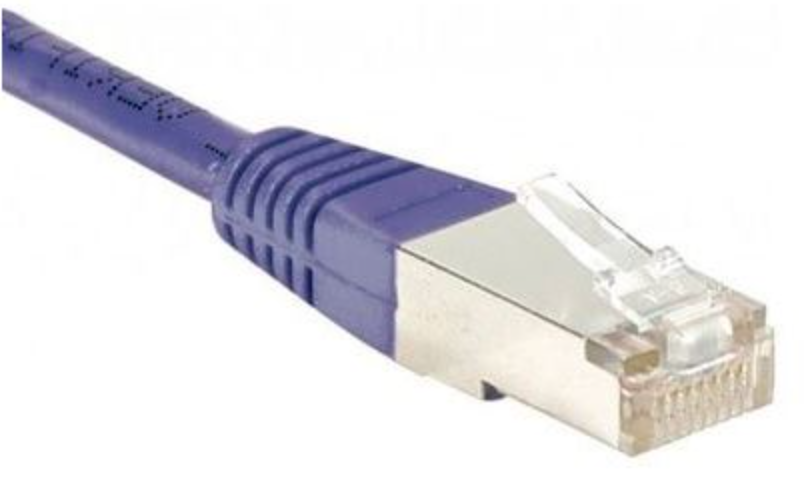
\includegraphics[scale=.5]{images/RJ45}
\caption{connecteur d'un câble RJ45}
\end{center}
\end{figure}

\begin{exercice}
Quels types d'appareils sont fréquemment connectés par ce type de câble?
\end{exercice}


\subsubsection{L'USB}



L'USB ({\it Universal Serial Bus}) est une norme de bus informatique permettant de connecter des appareils entre eux. Aujourd'hui, l'USB-C est le connecteur utilisé sur tous les appareils et peut être adapté pour recevoir d'autre type de connecteurs. 




Les câbles avec des connecteurs USB transmettent les données par signal électrique. Le débit théorique de ces câbles dépend du type du connecteur:
\begin{enumerate}
\item Type 1: jusqu'à 12 Mbit/s (1996)
\item Type 2: jusqu'à 480 Mbit/s (2000)
\item Type 3: jusqu'à 4.8 Gbit/s (2008)
\item Type 3.1: jusqu'à 10 Gbit/s
\item Type 4: jusqu'à 40 Gbit/s (2017)
\end{enumerate}

\begin{figure}[h]
\begin{center}
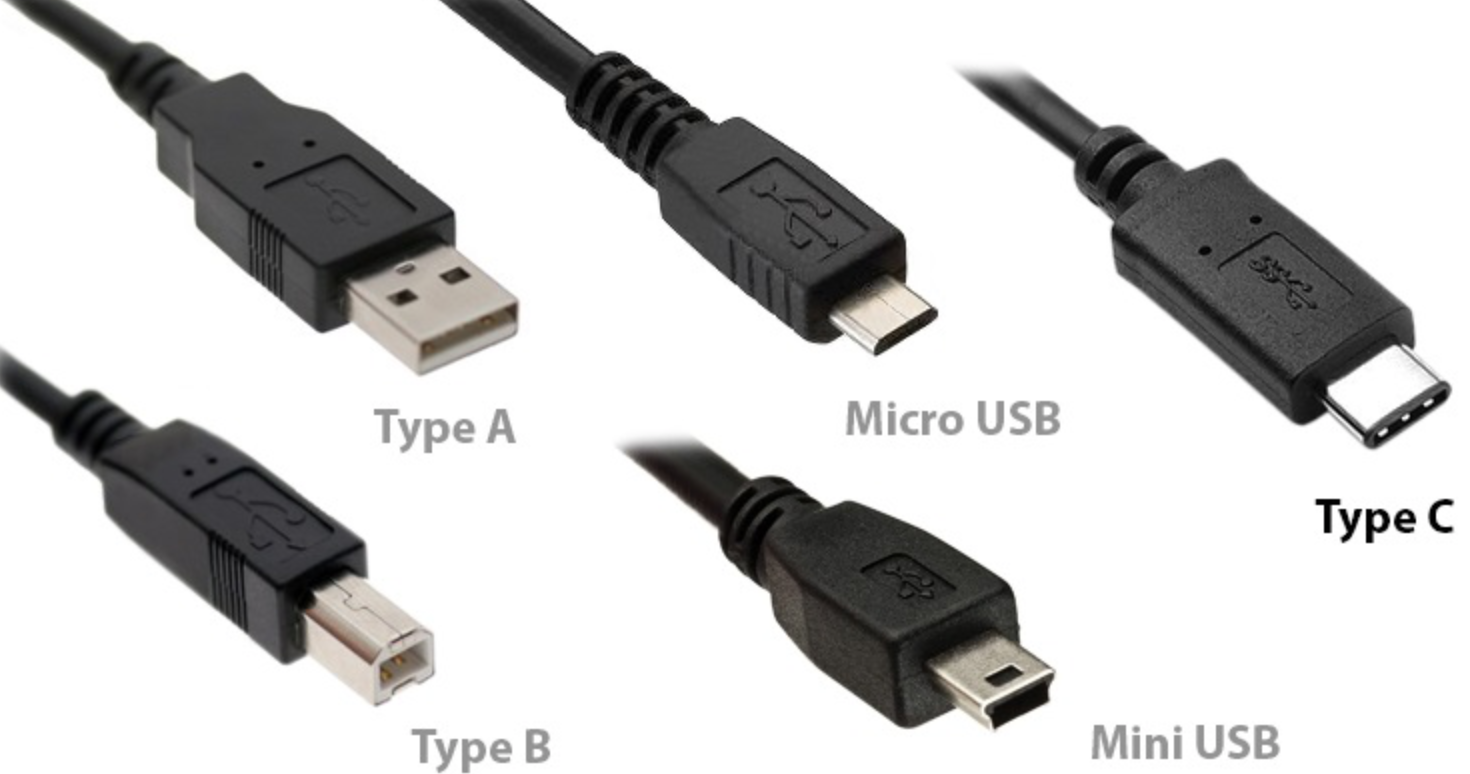
\includegraphics[scale=.4]{images/usb}
\caption{Les différents types de connecteur USB}
\end{center}
\end{figure}

\begin{exercice}
Quel est l'usage le plus fréquent des câbles USB?
\end{exercice}



\subsubsection{La fibre optique}

La fibre optique est un petit "câble" en verre ou en plastique dans lequel un rayon lumineux "rebondit". L'information est transmise par un signal lumineux.

Les avantages de la fibre optique sont:
\begin{enumerate}
\item Sa très faible perte de débit sur de longues distances.
\item Sa durée de vie (plus de 100 ans).
\item Une connexion Internet particulière plus rapide (jusqu'à 1 GB/s)
\end{enumerate}

Son principal désavantage est qu'elle est plutôt fragile et plus vulnérable aux dommages que peuvent l'être les fils de cuivre.

% image ajouté par edba le 18.04.2022
\begin{figure}[h]
\begin{center}
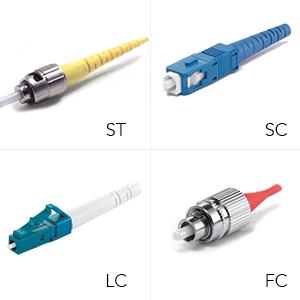
\includegraphics[scale=.5]{images/connecteurs-fibre-optique.png}
\caption{Les connecteurs optiques les plus utilisés}
\end{center}
\end{figure}


% complété par edba le 18.04.2022
\begin{remarque}
Début 2021, l'entreprise Google a mis en activité son nouveau câble de fibre optique reliant l'Europe aux Etats-Unis, soit 6'400 km de câble. Ce câble a un débit de 250 Tbits/s soit 250 000 Gbit/s. Il existe des milliers câbles sous-marins dans le monde. Certains sites les recensent  comme par exemple: https://www.infrapedia.com/app
\end{remarque}



%%%%%%%%%%%%%%%%%%%%%%%%%%%%%%%%%%%%%%%%%%%%%%%%%%%

\subsection{Les supports aériens}

\begin{defi}
Les {\bf supports aériens} envoient les données entre machines à travers d'antennes qui jouent le rôle d'émetteurs/receveurs. L'information est envoyée sous la forme d'ondes radio ou d'ondes  électromagnétiques. Les supports aériens permettent les communications d'un point vers plusieurs à la fois. On appelle cela une {\bf diffusion broadcast}.
\end{defi}


\begin{remarque}
La connexion par supports aériens demande plus de sécurité car il est plus facile d'{\it intercepter} la communication entre deux appareils ou de se connecter à un router Wi-Fi afin de bénéficier de sa connexion. 
\end{remarque}

\subsubsection{Wi-Fi}

Le Wi-Fi est un ensemble de protocoles (ou de règles) permettant la communication sans fil d'appareils. Un réseau particulier avec un router Wi-Fi est un bon exemple de réseau en étoile où tous les appareils d'une habitation sont reliés au même dispositif. 

La vitesse de connexion d'un routeur Wi-Fi dépend de sa norme:
\begin{enumerate}
\item la première norme, la 802.11b (1999): 11 Mbit/s.
\item la norme 802.11g (2003): 54 Mbit/s.
\item la norme 802.11ac (2013): 1,3 Gbit/s.
\item la norme 802.11ax (2021): 10,5 Gbit/s
\item la norme 802.11be (futur norme): En cours de définition
\end{enumerate}
La norme 802.11ax est la dernière norme 802.11 officielle. La distance du réseau dépend aussi de la norme. La dernière norme offre une portée de 70 mètres.

\begin{remarque}
La distance a un fort impact sur le débit du Wi-Fi. Pour y remédier, il faut augmenter la couverture du réseau en utilisant par exemple des répéteurs (appareils qui prennent le signal Wi-Fi et le répètent plus intensément). 
\end{remarque}

\subsubsection{4G - 5G}

La 4G et la 5G sont les 4e et 5e générations des standards pour la téléphonie mobile. La 4G a remplacé la 3G au début des années 2000 et a permis une multiplication par 500 du débit (1 Gb/s). 

L'augmentation du nombre d'appareils connectés rend la 4G obsolète. Elle sera petit à petit remplacée par la 5G qui offre un débit 100 fois plus rapide que la 4G.

\subsubsection{Autres supports aériens}

On peut citer l'infrarouge, le bluetooth (jusqu'à 54 Mbit/s pour la dernière norme), ou les connexions satellites comme autres support aériens.





%%%%%%%%%%%%%%%%%%%%%%%%%%%%%%%%%%%%%%%%%%%%%%%%%%%
%%%%%%%%%%%%%%%%%%%%%%%%%%%%%%%%%%%%%%%%%%%%%%%%%%%

\section{La Communication dans les réseaux}

%%%%%%%%%%%%%%%%%%%%%%%%%%%%%%%%%%%%%%%%%%%%%%%%%%%

\subsection{Les types de nœuds dans un réseau}

Dans un réseau, différents appareils sont connectés entre eux. Au niveau du graphe représentant ce réseau, ils correspondent aux nœuds. Ces nœuds sont de différentes natures.

\subsubsection{Ordinateurs personnels}

Le nœud le plus évident est l'{\bf ordinateur personnel} puisque c'est avec celui-ci que l'utilisateur rentre dans le réseau. Dans cette catégorie, on retrouve les ordinateurs de bureaux, les ordinateurs portables, les tablettes, les smartphones...

\subsubsection{Les périphériques}

D'autres types de nœud couramment rencontrés sont les {\bf périphériques}. Les périphériques permettent principalement d'accomplir une tâche demandée par un ordinateur personnel. Dans cette catégorie, on retrouve les imprimantes, les photocopieuses, les scanners, les caméras de surveillance, les vidéo-projecteurs...

\subsubsection{Les routeurs}

Moins visible par l'utilisateur mais essentiel au bon fonctionnement du réseau, le {\bf routeurs} est, comme son nom l'indique, l'appareil qui va établir les routes pour que les données arrivent au bon endroit. Cependant, un routeur n'a qu'une information limitée. Il ne connaît que ses voisins directs et ne sait pas ce qu'il se passe au-delà d'eux. 



%%%%%%%%%%%%%%%%%%%%%%%%%%%%%%%%%%%%%%%%%%%%%%%%

\subsection{Activité de groupes}

\begin{center}
\begin{tikzpicture}[scale=.85]

\def\long{.3};

\coordinate (A) at (3,4);
\coordinate (B) at (8,4);
\coordinate (C) at (2,8);
\coordinate (D) at (9,8);
\coordinate (E) at (3,12);
\coordinate (F) at (8,12);

\coordinate (AA) at (1,0);
\coordinate (AB) at (3,0);
\coordinate (AC) at (5,0);
\coordinate (AD) at (5,2);
\coordinate (AE) at (3,2);
\coordinate (AF) at (1,2);

\coordinate (BA) at (7,1);
\coordinate (BB) at (8,2);
\coordinate (BC) at (10,2);
\coordinate (BD) at (10,4);

\coordinate (CA) at (0,5);
\coordinate (CB) at (0,7);
\coordinate (CC) at (0,9);

\coordinate (FA) at (10,13);
\coordinate (FB) at (10,15);
\coordinate (FC) at (12,13);
\coordinate (FD) at (12,15);

\coordinate (EA) at (3,14);
\coordinate (EB) at (1,14);
\coordinate (EC) at (0,13);
\coordinate (ED) at (0,11);

\coordinate (PA) at (0,4);
\coordinate (PB) at (10,6);
\coordinate (PC) at (11,8);
\coordinate (PD) at (11,10);
\coordinate (PE) at (4,9);

%legende
\coordinate (triangle) at (0,-1);
\coordinate (rond) at (0,-2);
\coordinate (carre) at (0,-3);

\draw (E) -- (F);
\draw (C) -- (D) -- (F)
	(E) -- (C)
	(C) -- (B)
	(A) -- (D)
	(AA) -- (AB) -- (AC) -- (AD) -- (AE) -- (AF) -- (AA)
	(A) -- (AE)
	(B) -- (BA)
	(B) -- (BB)
	(B) -- (BC)
	(B) -- (BD)
	(C) -- (CA)
	(C) -- (CB)
	(C) -- (CC)
	(F) -- (FA) -- (FB) -- (FC) -- (FD) -- (FA)
	(FB) -- (FD)
	(FA) -- (FC)
	(E) -- (EA)
	(E) -- (EB)
	(E) -- (EC)
	(E) -- (ED)
	(PA) -- (CA)
	(D) -- (PB)
	(D) -- (PC)
	(D) -- (PD)
	(C) -- (PE);


%tracer des carrés
\foreach \x in {(A),(B),(C),(D),(E),(F),(carre)}
	\filldraw[fill=lightgray] \x ++(-\long,-\long) rectangle ++(2*\long,2*\long);
	
%tracé des cercle	
\foreach \x in {(AA),(AB),(AC),(AD),(AE),(AF),
						(BA),(BB),(BC),(BD),
						(CA),(CB),(CC),
						(FA),(FB),(FC),(FD),
						(EA),(EB),(EC),(ED),
						(rond)}
	\filldraw[fill=lightgray] \x circle (\long);


%tracé des triangles
\foreach \x in {(PA),(PB),(PC),(PD),(PE),(triangle)}
	\filldraw[fill=lightgray] \x ++(-\long,-\long) -- ++(2*\long, 0) -- ++(-\long,1.6*\long) -- cycle;
,
\draw (carre) +(.5,0) node[anchor=west] {: routeurs} ;
\draw (triangle) +(0.5,0) node[anchor=west] {: périphériques} ;
\draw (rond) +(.5,0) node[anchor=west] {: ordinateurs} ;

\end{tikzpicture}

\end{center}


Par groupe de 3 ou 4 élèves, prendre connaissance de la situation suivante puis répondre aux différentes questions:

\ 

Le graphe ci-dessus représente le réseau d'une entreprise, avec des ordinateurs de travail (représentés par des cercles), des routeurs (représentés par des carrés) et des périphériques (représentés par des triangles).

\newpage

{\bf Question 1:} Quels types de sous-réseaux reconnaissez vous dans ce graphe? 

\vskip+3cm

{\bf Question 2:} Quels types de périphériques peuvent représenter les triangles?

\vskip+3cm

{\bf Question 3:} Quel est le rôle d'un routeur?

\vskip+3cm


{\bf Question 4:} Quelle connaissance du réseau possède chaque routeur, c'est à dire, combien d'autres appareils du réseau connaît-il?

\vskip+3cm

{\bf Question 5:} Chaque ordinateur du réseau doit pouvoir envoyer des informations à n'importe quel autre ordinateur du réseau et recevoir une réponse en échange. Quel ensemble de règles doit respecter ce réseau pour que cela soit possible?

\vskip+3cm

\newpage



%%%%%%%%%%%%%%%%%%%%%%%%%%%%%%%%%%%%%%%%%%%%%%%%

\subsection{Les protocoles}

L'activité a montré que pour avoir une communication fiable entre les ordinateurs d'un réseau, il faut avoir les mêmes règles communes pour que tout le monde puisse se comprendre. C'est ce que nous appelons un {\bf protocole}.

\begin{defi}
Un {\bf protocole de communication} est un ensemble de règles qui décrivent comment la communication entre deux parties doit se faire à travers un réseau.

\end{defi}

Ces protocoles sont essentiels dans le cas de l'informatique car la communication passe par des ordinateurs. La juste programmation du protocole dans chaque ordinateur devrait garantir la bonne transmission des informations.

\begin{remarques}
\begin{enumerate}
\item[]
\item Le code de la route d'un pays peut-être considéré comme un protocole. C'est un ensemble de règles qui permet d'éviter les accidents.
\item En informatique, les protocoles les plus connus sont l'{\it Internet Protocol (IP)} qui permet l'adressage des ordinateurs et l'{\it HyperText Transfer Protocol (http)} qui permet de mettre en relation des clients avec des serveurs contenant des sites web.

\end{enumerate}

\end{remarques}

%%%%%%%%%%%%%%%%%%%%%%%%%%%%%%%%%%%%%%%%%%%%%%%%

\subsection{L'adressage}

Le premier point à respecter, pour qu'un réseau fonctionne correctement consiste à attribuer à chaque appareil sur le réseau un unique identifiant, qu'on appelle l'adresse. Pour cela on utilise une adresse {\it IP}. 

\begin{defi}
Le {\bf Protocol Internet (IP)} permet l'adressage unique des terminaux connectés à Internet. À chaque terminal est associé une adresse {\it unique} de la forme 134.23.112.20 (4 nombres entre 0 et 255 et séparés par un point). 
\end{defi} 


\begin{remarques}
\begin{enumerate}
\item[]
\item Le type d'adresse actuelle est l'IPv4. Mais l'augmentation du nombre de terminaux pousse à un nouveau type d'adressage, l'IPv6 permettant de générer beaucoup plus d'adresses.
\item Une adresse IP est donnée par l'ICANN (Internet Corporation for Assigned Names and Numbers).
\end{enumerate}
\end{remarques}

%%%%%%%%%%%%%%%%%%%%%%%%%%%%%%%%%%%%%%%%%%%%%%%%

\subsection{Le routage}

Un {\bf routeur} est un terminal qui reçoit des données et les dirige dans la bonne direction afin que ces données arrivent à destination. Un routeur ne connaît que ses voisins directs, ceux avec lesquels il peut communiquer. Il n'a pas connaissance de tout le réseau et il ne choisit pas la prochaine destination en essayant d'optimiser le parcours le plus efficace. Pour choisir la où il va envoyer la donnée qu'il a reçu, le routeur utilise une {\bf table de routage}.

\begin{defi}
Une {\bf table de routage} est une base de données utilisée par un ordinateur ou un routeur qui associe des adresses IP ou des préfixes d'adresses IP à des adresses appartenant au sous-réseau de l'ordinateur ou du routeur correspondant aux terminaux auxquels il est directement connecté.
\end{defi}

Dans l'exemple suivant, on utilise un réseau ou les adresses sont simplifiées et son représentées par des paires de lettres: 

\begin{center}
\begin{tikzpicture}

\def\long{.4};

\coordinate (AA) at (1,0);
\coordinate (AB) at (0,2);
\coordinate (A0) at (2,2);

\coordinate (BA) at (6,0);
\coordinate (BB) at (8,2);
\coordinate (B0) at (6,2);
\coordinate (BC) at (8,0);

\coordinate (CA) at (3,7);
\coordinate (CB) at (5,7);
\coordinate (C0) at (4,5);

\draw (AB) -- (A0) -- (AA)
	(BC) -- (BA) -- (B0) -- (BB) -- (BA)
	(CA) -- (C0) -- (CB)
	(A0) -- (B0) -- (C0) -- cycle;
	
	\draw[dashed] (CA) -- (-1,7)
		(C0) -- (-1,4)
		(CB) -- (9,7)
		(AB) -- (-1,2)
		(A0) -- (-1,-1)
		(AA) -- ++(0,-1)
		(B0) --  (4,-1)
		(BA) -- ++(1,-1)
		(BC) -- ++(2,-1)
		(BB) -- ++(1,-1);

\foreach \x in {(A0),(B0),(C0)}
	\filldraw[fill=lightgray] \x ++(-\long,-\long) rectangle ++(2*\long,2*\long);
	
\foreach \x in {A0,B0,C0}
	\draw (\x) node {\x};
	
\filldraw[fill=lightgray] (BC) ++(-\long,-\long) -- ++(2*\long,0) -- ++(-\long, 1.8*\long) -- cycle;

\foreach \x in {(AA),(AB),(BA),(BB),(CA),(CB)}
	\filldraw[fill=lightgray] \x circle (\long);
	
\draw (AA) node {AA};
\draw (AB) node {AB};
\draw (BA) node {BA};
\draw (BB) node {BB};
\draw (CA) node {CA};
\draw (CB) node {CB};
\draw (BC) ++(0,-.2) node {BC};

\begin{scope}[shift={(0,-1)}] %table AA
\draw (0,0) -- (2,0) -- (2,-2) -- (0,-2) -- cycle
	(1,0) -- (1,-2)
	(0,-.5) -- (2,-.5)
	(0,-1) -- (2,-1)
	(0,-1.5) -- (2,-1.5)
	(0.5,-.3) node {A-}    (1.5,-.3) node {A0}
	(0.5,-.8) node {B-}    (1.5,-.8) node {A0}
	(0.5,-1.3) node {C-}    (1.5,-1.3) node {A0}
	(0.5,-1.8) node {}    (1.5,-1.8) node {} ;
\end{scope}

\begin{scope}[shift={(-3,-1)}] %table A0
\draw (0,0) -- (2,0) -- (2,-2) -- (0,-2) -- cycle
	(1,0) -- (1,-2)
	(0,-.5) -- (2,-.5)
	(0,-1) -- (2,-1)
	(0,-1.5) -- (2,-1.5)
	(0.5,-.3) node {AA}    (1.5,-.3) node {AA}
	(0.5,-.8) node {AB}    (1.5,-.8) node {AB}
	(0.5,-1.3) node {B-}    (1.5,-1.3) node {B0}
	(0.5,-1.8) node {C-}    (1.5,-1.8) node {C0} ;
\end{scope}

\begin{scope}[shift={(-3,2)}] %table AB
\draw (0,0) -- (2,0) -- (2,-2) -- (0,-2) -- cycle
	(1,0) -- (1,-2)
	(0,-.5) -- (2,-.5)
	(0,-1) -- (2,-1)
	(0,-1.5) -- (2,-1.5)
	(0.5,-.3) node {A-}    (1.5,-.3) node {A0}
	(0.5,-.8) node {B-}    (1.5,-.8) node {A0}
	(0.5,-1.3) node {C-}    (1.5,-1.3) node {A0}
	(0.5,-1.8) node {}    (1.5,-1.8) node {} ;
\end{scope}
	
	
\begin{scope}[shift={(3,-1)}] %table B0
\draw (0,0) -- (2,0) -- (2,-2.5) -- (0,-2.5) -- cycle
	(1,0) -- (1,-2.5)
	(0,-.5) -- (2,-.5)
	(0,-1) -- (2,-1)
	(0,-1.5) -- (2,-1.5)
	(0,-2) -- (2,-2)
	(0.5,-.3) node {BB}    (1.5,-.3) node {BB}
	(0.5,-.8) node {BA}    (1.5,-.8) node {BA}
	(0.5,-1.3) node {C-}    (1.5,-1.3) node {C0}
	(0.5,-1.8) node {B-}    (1.5,-1.8) node {B0}
	(0.5,-2.3) node {BC}    (1.5,-2.3) node {BA} ;
\end{scope}

\begin{scope}[shift={(6,-1)}] %table BA
\draw (0,0) -- (2,0) -- (2,-2) -- (0,-2) -- cycle
	(1,0) -- (1,-2)
	(0,-.5) -- (2,-.5)
	(0,-1) -- (2,-1)
	(0,-1.5) -- (2,-1.5)
	(0.5,-.3) node {BB}    (1.5,-.3) node {BB}
	(0.5,-.8) node {BC}    (1.5,-.8) node {BC}
	(0.5,-1.3) node {Def.}    (1.5,-1.3) node {B0}
	(0.5,-1.8) node {}    (1.5,-1.8) node {} ;
\end{scope}
	
\begin{scope}[shift={(9,-1)}] %table BC
\draw (0,0) -- (2,0) -- (2,-2) -- (0,-2) -- cycle
	(1,0) -- (1,-2)
	(0,-.5) -- (2,-.5)
	(0,-1) -- (2,-1)
	(0,-1.5) -- (2,-1.5)
	(0.5,-.3) node {Def.}    (1.5,-.3) node {BA}
	(0.5,-.8) node {}    (1.5,-.8) node {}
	(0.5,-1.3) node {}    (1.5,-1.3) node {}
	(0.5,-1.8) node {}    (1.5,-1.8) node {} ;
\end{scope}

\begin{scope}[shift={(9,2)}] %table BB
\draw (0,0) -- (2,0) -- (2,-2) -- (0,-2) -- cycle
	(1,0) -- (1,-2)
	(0,-.5) -- (2,-.5)
	(0,-1) -- (2,-1)
	(0,-1.5) -- (2,-1.5)
	(0.5,-.3) node {BA}    (1.5,-.3) node {BA}
	(0.5,-.8) node {Def.}    (1.5,-.8) node {B0}
	(0.5,-1.3) node {}    (1.5,-1.3) node {}
	(0.5,-1.8) node {}    (1.5,-1.8) node {} ;
\end{scope}



\begin{scope}[shift={(-3,5)}] %table C0
\draw (0,0) -- (2,0) -- (2,-2) -- (0,-2) -- cycle
	(1,0) -- (1,-2)
	(0,-.5) -- (2,-.5)
	(0,-1) -- (2,-1)
	(0,-1.5) -- (2,-1.5)
	(0.5,-.3) node {CA}    (1.5,-.3) node {CA}
	(0.5,-.8) node {CB}    (1.5,-.8) node {CB}
	(0.5,-1.3) node {A-}    (1.5,-1.3) node {A0}
	(0.5,-1.8) node {B-}    (1.5,-1.8) node {B0} ;
\end{scope}

\begin{scope}[shift={(-3,8)}] %table CA
\draw (0,0) -- (2,0) -- (2,-2) -- (0,-2) -- cycle
	(1,0) -- (1,-2)
	(0,-.5) -- (2,-.5)
	(0,-1) -- (2,-1)
	(0,-1.5) -- (2,-1.5)
	(0.5,-.3) node {C-}    (1.5,-.3) node {C0}
	(0.5,-.8) node {B-}    (1.5,-.8) node {C0}
	(0.5,-1.3) node {A-}    (1.5,-1.3) node {C0}
	(0.5,-1.8) node {}    (1.5,-1.8) node {} ;
\end{scope}

\begin{scope}[shift={(9,8)}] %table CC
\draw (0,0) -- (2,0) -- (2,-2) -- (0,-2) -- cycle
	(1,0) -- (1,-2)
	(0,-.5) -- (2,-.5)
	(0,-1) -- (2,-1)
	(0,-1.5) -- (2,-1.5)
	(0.5,-.3) node {C-}    (1.5,-.3) node {C0}
	(0.5,-.8) node {B-}    (1.5,-.8) node {C0}
	(0.5,-1.3) node {A-}    (1.5,-1.3) node {C0}
	(0.5,-1.8) node {}    (1.5,-1.8) node {} ;
\end{scope}

	

\end{tikzpicture}
\end{center}


À chaque routeur, ordinateur ou périphérique est associé sa table de routage. Dans cette table, la colonne de gauche correspond à l'adresse de destination (ou à un préfixe d'adresse de destination) du paquet de données. L'adresse à droite est l'adresse du terminal auquel il faut envoyer ce paquet (ce qui est appelé le {\bf next-hop}).

Dans la table de routage il faut souvent indiquer une route {\it par défaut}, c'est à dire le routeur auquel envoyer un paquet dont l'adresse de destination n'apparaît pas dans les adresses de la table de routage.  Dans notre exemple, cela est signifié par un {\it Def.}.

\begin{exercice}
Déterminer le chemin parcouru par une information :
\begin{enumerate}
\item allant de CA à BC.
\item allant de BA à AB.
\end{enumerate}
\end{exercice}

\newpage

\begin{exercice}
Dans le diagramme de l'activité de groupe de la section 1.5.2, établir un adressage cohérent de tous les terminaux puis établir les tables de routage afin que chaque terminal du réseau puisse communiquer avec un autre terminal du réseau.


\begin{center}
\begin{tikzpicture}[scale=1.1]

\def\long{.3};

\coordinate (A) at (3,4);
\coordinate (B) at (8,4);
\coordinate (C) at (2,8);
\coordinate (D) at (9,8);
\coordinate (E) at (3,12);
\coordinate (F) at (8,12);

\coordinate (AA) at (1,0);
\coordinate (AB) at (3,0);
\coordinate (AC) at (5,0);
\coordinate (AD) at (5,2);
\coordinate (AE) at (3,2);
\coordinate (AF) at (1,2);

\coordinate (BA) at (7,1);
\coordinate (BB) at (8,2);
\coordinate (BC) at (10,2);
\coordinate (BD) at (10,4);

\coordinate (CA) at (0,5);
\coordinate (CB) at (0,7);
\coordinate (CC) at (0,9);

\coordinate (FA) at (10,13);
\coordinate (FB) at (10,15);
\coordinate (FC) at (12,13);
\coordinate (FD) at (12,15);

\coordinate (EA) at (3,14);
\coordinate (EB) at (1,14);
\coordinate (EC) at (0,13);
\coordinate (ED) at (0,11);

\coordinate (PA) at (0,4);
\coordinate (PB) at (10,6);
\coordinate (PC) at (11,8);
\coordinate (PD) at (11,10);
\coordinate (PE) at (4,9);

%legende
\coordinate (triangle) at (0,-1);
\coordinate (rond) at (0,-2);
\coordinate (carre) at (0,-3);

\draw (E) -- (F);
\draw (C) -- (D) -- (F)
	(E) -- (C)
	(C) -- (B)
	(A) -- (D)
	(AA) -- (AB) -- (AC) -- (AD) -- (AE) -- (AF) -- (AA)
	(A) -- (AE)
	(B) -- (BA)
	(B) -- (BB)
	(B) -- (BC)
	(B) -- (BD)
	(C) -- (CA)
	(C) -- (CB)
	(C) -- (CC)
	(F) -- (FA) -- (FB) -- (FC) -- (FD) -- (FA)
	(FB) -- (FD)
	(FA) -- (FC)
	(E) -- (EA)
	(E) -- (EB)
	(E) -- (EC)
	(E) -- (ED)
	(PA) -- (CA)
	(D) -- (PB)
	(D) -- (PC)
	(D) -- (PD)
	(C) -- (PE);


%tracer des carrés
\foreach \x in {(A),(B),(C),(D),(E),(F),(carre)}
	\filldraw[fill=lightgray] \x ++(-\long,-\long) rectangle ++(2*\long,2*\long);
	
%tracé des cercle	
\foreach \x in {(AA),(AB),(AC),(AD),(AE),(AF),
						(BA),(BB),(BC),(BD),
						(CA),(CB),(CC),
						(FA),(FB),(FC),(FD),
						(EA),(EB),(EC),(ED),
						(rond)}
	\filldraw[fill=lightgray] \x circle (\long);


%tracé des triangles
\foreach \x in {(PA),(PB),(PC),(PD),(PE),(triangle)}
	\filldraw[fill=lightgray] \x ++(-\long,-\long) -- ++(2*\long, 0) -- ++(-\long,1.6*\long) -- cycle;
,
\draw (carre) +(.5,0) node[anchor=west] {: routeurs} ;
\draw (triangle) +(0.5,0) node[anchor=west] {: périphériques} ;
\draw (rond) +(.5,0) node[anchor=west] {: ordinateurs} ;

\end{tikzpicture}

\end{center}

\end{exercice}


%%%%%%%%%%%%%%%%%%%%%%%%%%%%%%%%%%%%%%%%%%%%%%%%
%%%%%%%%%%%%%%%%%%%%%%%%%%%%%%%%%%%%%%%%%%%%%%%%

\section{Les protocoles}

Nous rappelons la définition suivante:

\begin{defi}
Un {\bf protocole de communication} est un ensemble de règles qui décrivent comment la communication entre deux parties doit se faire à travers un réseau.

\end{defi}

Ces protocoles sont importants car les échanges sur les réseaux sont principalement fait par des machines.

\subsection{Hiérarchies de protocoles}

Les protocoles informatiques servent à définir:
\begin{enumerate}
\item comment doit être encodée l'information pour être transmise à travers un support spécifique;
\item quel type d'information doit être attaché à un message pour qu'il soit acheminé/routé correctement;
\item l'ordre dans lequel les messages doivent être envoyés entre des machines pour qu'elles puissent se comprendre.

\end{enumerate}

C'est pour cela que nous avons besoin d'une hiérarchie de protocoles de réseaux:

\begin{defi}
Une {\bf hiérarchie de protocoles de réseaux} décrit les différents niveaux d'abstraction des protocoles qui sont utilisés dans un moyen de communication. Ces niveaux sont représentés par des {\bf couches} empilées les unes au-dessus des autres.
\end{defi}

L'objectif de chaque couche est de fournir un service à celle qui se trouve au-dessus en d'elle cachant les détails de comment a été implémentée la fonctionnalité offerte.

\subsection{Exemple concret}

Pour envoyer un courrier à un ami dans le monde il faut un ensemble de règles communes afin que cela puisse se dérouler sans problème:

\begin{enumerate}
\item Premièrement, il faut un réseau postal qui va pouvoir acheminer la lettre de l'émetteur jusqu'au destinataire. C'est le {\bf réseau physique} composé de voies, de routes, et utilisant des trains, des avions, des vélos...
\item Il faut ensuite un ensemble de règles permettant à chaque lieu où passera la lettre de savoir comment elle sera acheminée au lieu suivant.

 Par exemple, le facteur sait qu'il doit apporter les lettres de la boite de dépôt au centre de triage. Le centre de triage sait que les lettres pour l'Amérique doivent être mise dans un sac postal et prendre tel avion...
 
 C'est ce que nous appelons la {\bf la couche de liaison de données}. 
 
 \item Selon l'adresse écrite dessus, les différents centres de triage vont envoyer la lettre à d'autres centres de triage afin d'acheminer le courrier. C'est {\bf la couche réseau}.
 
 \item Un ensemble de règles doit établir si les lettres arrivent bien à destination, s'il faut réorganiser les flux postaux ou gérer des problèmes dans certains centres de triage. C'est {\bf la couche transport}.
 
 \item Pour bien se comprendre, l'émetteur et le destinataire doivent se mettre d'accord sur le langage utilisé dans la lettre. Un format d'écriture de l'adresse doit aussi être respecté. Enfin, l'émetteur doit aller poser la lettre sur le réseau afin qu'elle soit acheminée. C'est {\bf la couche application}. 
 \end{enumerate}


\subsection{Hiérarchie standard}

De la même façon, nous pouvons retrouver un ensemble de règles permettant qu'une information soit envoyée d'un ordinateur ou d'un serveur vers un destinataire. 

\begin{enumerate}
\item {\bf La couche physique} est l'ensemble des connexions reliant tous les terminaux du réseau. La connexion peut être par exemple un câble ou un réseau sans fil.
\item {\bf La couche de liaison de données} est l'ensemble des règles permettant la communication entre deux terminaux connectés. Un exemple de règles est le protocole Ethernet permettant de relier deux ordinateurs entre eux. Cette couche est aussi la couche qui vérifie s'il y a des erreurs de transmission de données. 

\item {\bf La couche réseau} comprend l'ensemble des règles de routage permettant à l'information de circuler de l'émetteur jusqu'au destinataire le plus rapidement possible.

\item {\bf La couche transport} vérifie que les informations arrivent bien à destination, sans erreur et dans le bon ordre.

\item {\bf La couche application} est l'ensemble des protocoles utilisées par les applications utilisateurs d'un réseau pour se comprendre. Elle définit donc le format des messages envoyés entre applications. 


\end{enumerate}

\begin{exercice}
Dans quelle couche placeriez-vous ces différentes situations?
\begin{enumerate}
\item Le temps que doit mettre un train pour aller d'une ville à une autre et le nombre de passagers qu'il peut prendre.
\item L'ensemble des autoroutes espagnoles.
\item La gestion du réseau électrique Suisse et la garantie que chaque foyer ait de l'électricité.
\item Les formules de politesse lorsque nous envoyons un e-mail à un supérieur hiérarchique.
\item L'acheminement de l'eau lorsque j'ouvre le robinet.

\end{enumerate}
\end{exercice}

\subsection{Exemple de protocole: le client-serveur}

\begin{defi}
Un protocole ou environnement {\bf client-serveur} est un mode de communication entre plusieurs programmes ou processus: l'un est appelé le {\bf client} qui envoie des requêtes, et l'autre un {\bf serveur} qui attend les requêtes des clients et qui y répond. Le serveur offre un {\bf service} au client. 
\end{defi}

Les serveurs ont donc une puissance de calcul, un ensemble d'entrées et de sorties et une connexion réseau bien plus importante qu'un ordinateur personnel afin de pouvoir gérer les nombreuses requêtes des clients.

Afin de communiquer, le client et le serveur doivent utiliser le même protocole de communication. Les exemples de protocole client-serveur sont:
\begin{enumerate}
\item un serveur web publie des pages demandées par des navigateurs web (les clients);
\item un serveur de messagerie électronique transmets les e-mails demandés par des clients de messagerie (outlook, mail, thunderbird,...)
\item un système {\bf pair à pair } (peer-to-peer en anglais) est un environnement client-serveur ou chaque programme peut être client ou serveur. Le programme est client lorsqu'il demande et récupère des données, et devient serveur lorsqu'il fournit des données.
\end{enumerate}

\vskip1cm

Le principe de fonctionnement du modèle est le suivant:
\begin{enumerate}[i)]
\item Lorsqu'un client veut accéder à une ressource stockée sur un serveur donné (une page web, une image ou une vidéo, par exemple), il envoie à ce dernier une {\it requête} qui spécifie  le nom
ou l'identifiant de la ressource à lui transmettre.
\item Lorsque le serveur reçoit la requête, il recherche la ressource demandée dans son registre.
\item S'il la trouve, il envoie une {\it réponse} à la requête du client dans laquelle il inclut la ressource demandée, ainsi qu'un code de confirmation.
\item S'il ne possède pas la ressource ou qu'une autre erreur est rencontrée, il répond au client avec un code d'erreur qui lui indique le type de problème survenu au cours de leur échange.
\end{enumerate}


\vskip1cm

L'exemple le plus connu d'application de la couche 5 (couche application) qui utilise le modèle client-
serveur est le {\it World Wide Web} (souvent plus simplement appelé le {\it web}). Il correspond à un réseau international de serveurs qui hébergent les sites web que nous avons aujourd'hui tous l'habitude de consulter quotidiennement. Le web est souvent confondu à tort avec Internet. Internet correspond à un vaste réseau informatique d'envergure internationale qui utilise les protocoles des couches décrites dans ce chapitre pour permettre à des ordinateurs de communiquer entre eux. Le web n'est qu'un exemple d'application de la couche 5 qui utilise Internet pour échanger de l'information entre des utilisateurs. D'autres services utilisent Internet, comme l'e-mail, par exemple, ou encore les plate-formes de streaming vidéo, les jeux-vidéos multijoueurs, etc.



\subsection{Un  autre exemple de protocole: le DNS}


Nous avons vu que lorsqu'une machine souhaite envoyer un message à une autre, elle doit spécifier son adresse IP pour que l'information puisse être routée à travers le réseau. Toutefois, l'utilisation directe d'adresses IP présente plusieurs problèmes. Le premier est que ces dernières sont numériques et donc très difficiles à retenir pour les utilisateurs humains d'un réseau (imaginez s'il fallait entrer une adresse du type 192.168.22.1 dans notre navigateur à chaque fois que nous voulons accéder à notre site favori !). Une autre difficulté liée aux adresses IP est que dès qu'un service est déplacé d'une machine vers une autre, son adresse IP change. Par exemple, si un site hébergé sur un serveur doit être migré vers un autre pour des questions de maintenance, son adresse IP va changer et tous ses visiteurs devront en être informés pour pouvoir continuer à y accéder.

L'objectif du protocole DNS est d'associer des noms fixes aux machines connectées à Internet pour qu'elles puissent communiquer sans devoir directement utiliser leurs adresses IP. C'est donc ce protocole qui nous permet d'accéder quotidiennement à nos sites préférés avec des adresses comme {\it www.monsitefavori.com}, plutôt que de longues suites de chiffres difficiles à retenir.
Le principe de base du {\it Domain Name System} est le suivant :
\begin{itemize}
\item Lorsqu'une application souhaite accéder à un service avec un nom donné, elle envoie une
requête à un serveur DNS pour qu'il lui communique l'adresse IP associée à ce nom ;
\item Un serveur DNS est un serveur particulier qui maintient un registre associant des noms de domaines à leurs adresses IP. Quand ce serveur reçoit une requête, il recherche le nom demandé dans son registre et s'il trouve une correspondance, il répond avec l'adresse IP associée. Sinon, il retransmet la requête à un autre serveur DNS plus susceptible de connaître
la réponse, qui va effectuer la même tâche; soit trouver le nom recherché dans son registre, soit retransmettre la requête plus loin. Ces étapes sont répétées jusqu'à ce qu'un serveur qui connaît le nom recherché soit trouvé et retourne l'adresse IP désirée.
\end{itemize}







\end{document}


%% 2022 avril
%% TZ relecture et corrections de coquilles orthographiques 



